\documentclass[twoside, twocolumn, a4paper]{jarticle}

%
% is.sty は必要
\usepackage{is}  
%
%
%
% 以下各自が必要なパッケージは加えてよい. 
%
%\usepackage{rsfs}
\usepackage{amsmath}
\usepackage{stmaryrd}
\usepackage{amsfonts}
\usepackage{amssymb}
\usepackage{theorem}
% \usepackage{epsf}

% 自分で定義したマクロファイル
 % 型
\newcommand\Int{\textsf{int}}
\newcommand\Arrow[2]{{#1}\rightarrow{#2}}

% ラムダ式
\newcommand\Lam[2]{\lambda{#1}.\,{#2}}
\newcommand\LamP[2]{(\Lam{#1}{#2})}
\newcommand\App[2]{{#1}\,{#2}}
\newcommand\AppP[2]{(\App{#1}{#2})}
\newcommand\Shift[2]{{\cal S}{#1}.\,{#2}}
\newcommand\ShiftP[2]{(\Shift{#1}{#2})}
\newcommand\Reset[1]{\langle{#1}\rangle}

% Judgement
\newcommand\Judge[3]{{#1}\vdash{#2}:{#3}}

% CPS 変換
\newcommand\CPS[1]{[\![{#1]\!]}}


% 証明木を書く場合以下を読み込む
\usepackage{proof}

% 定理を使う場合、以下のようなものを書く
\newtheorem{definition}{定義}
\newtheorem{proposition}[definition]{命題}
\newtheorem{lemma}[definition]{補題}
\newtheorem{theorem}[definition]{定理}
% [...] 内に指定するとカウンタを共有する

%
% 以下を書き換えてタイトル部に
%------------------------------------------------------------
\title{{\gt{タイトル}}}
\author{{\gt 名前~~~~(指導教員:浅井 健一)}}
%------------------------------------------------------------

%
%
% ここから本体
%%%%%%%%%%%%%%%%%%%%%%%%%%%%%%%%%%%%%%%%%%
\begin{document}
%%%%%%%%%%%%%%%%%%%%%%%%%%%%%%%%%%%%%%%%%%
%
% 以下の3行は変更しない. 
%
\raggedbottom
\maketitle
\setlength{\baselineskip}{12.5pt}

%%%%%開始ページ数を設定する(この例では1)%%%%%%%%%%%
\setcounter{page}{1}

\setlength{\abovedisplayskip}{0pt}

\section{はじめに}

書いたプログラムが思った通りの挙動をしない時、プログラマはデバッグをする必要がある。

単純なデバッグはプログラムを実行した際の出力から推測したりソースコードを眺めることで行われるが、そのようなデバッグは「ソースコードのどの部分が間違っているか」を示すものが無く、多くの時間や労力を要することがある。特にプログラミングにまだ慣れていない初学者にとっては、デバッグの経験や言語に対する理解が乏しい為、より困難な作業になると考えられる。

そこで色々な言語にデバッガが用意されているが、デバッガを利用するには、デバッガのコマンドの文字列や意味を覚えたり、ブレイクポイントを設定する箇所を考えたりといった、初学者にとってやはり困難な操作が必要になる。また、一般的なデバッガで表示されるのは「ソースコード中の実行中の行」であり、どこで今の関数を呼び出されたのか、この後どんな計算があるのかなどといったプログラム全体の流れが分かりにくい。

\begin{figure}
  \begin{center}
    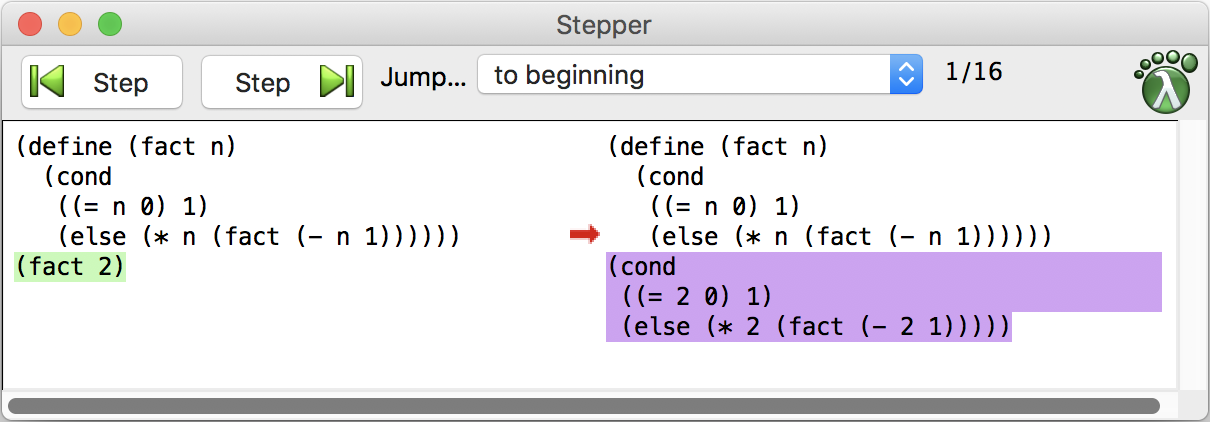
\includegraphics[width=13cm]{racket1.png}
  \end{center}
  \caption{DrRacket のステッパ}
  \label{figure:racket1}
\end{figure}

\begin{figure}
  \begin{center}
    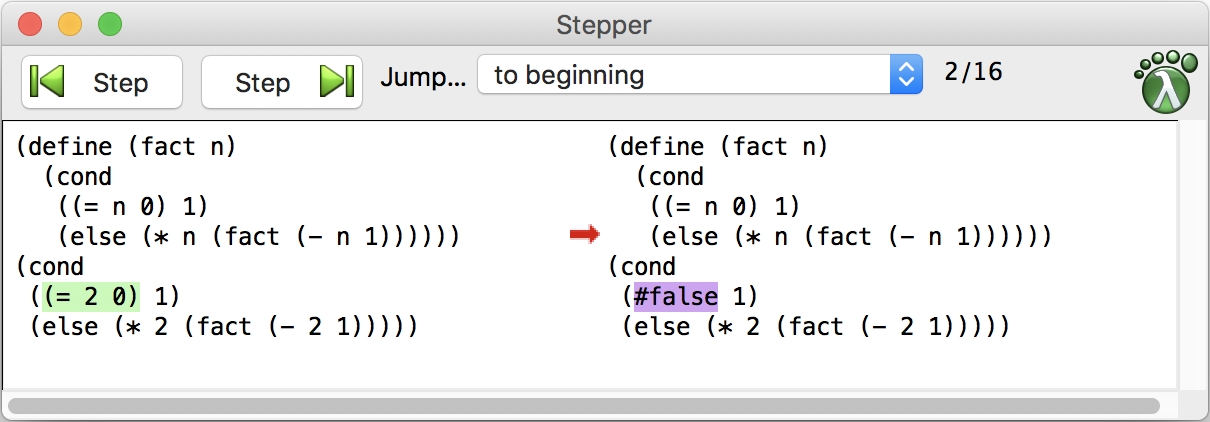
\includegraphics[width=13cm]{racket2.png}
  \end{center}
  \caption{DrRacket のステッパを進めた様子}
  \label{figure:racket2}
\end{figure}

我々は、プログラミング初心者がデバッグをするのに最適な方法は、ステッパを使うことだと考える。ステッパは Racket 言語の統合開発環境 DrRacket において提供されているツール\cite{clements01}である。ユーザがエディタにプログラムを書いてステッパ起動ボタンを押すと、図\ref{figure:racket1}のようなウインドウが表示される。図\ref{figure:racket1}は、再帰関数を用いて2の階乗を計算するプログラムを入力してステッパを起動したときの様子である。ウインドウには左右にそれぞれプログラムが表示されている。左はユーザが入力したプログラムと同じものであり、このプログラムで最初に簡約される式 \texttt{(fact 2)} が緑色にハイライトされている。右側のプログラムでは、ハイライトされた部分以外は左側と同じプログラムが表示されており、左側では緑色だった式 \texttt{(fact 2)} がその簡約結果に置き換えられ、紫色でハイライトされている。

Step ボタンのうち右の実行を進めるボタンを押すと図\ref{figure:racket2}のような表示に切り替わる。最初(図\ref{figure:racket1})は右側にあったプログラムと同じプログラムが左に表示され、次に簡約される部分式 \texttt{(= 2 0)} が緑色にハイライトされており、右側には同様にその部分が簡約されて紫色になったプログラムが表示されている。当初 \texttt{(fact 2)} だった式がその値である \texttt{2} になるステップまで、ボタンを押すと次々に簡約が行われてプログラムが変形していく様子を視覚的に見ることができる。

このように、プログラムを実行したときに、実行結果の値だけでなく、実行中にプログラムが代数的にどのように書き換えられていくかを見せるツールがステッパである。ステッパの操作は基本的に「前のステップへ」「次のステップへ」のボタンを押すのみであり、プログラミングや CUI での操作に慣れていない初心者でも使いやすい。

しかし、DrRacket のステッパが受け付けるのは Racket 言語のうちの一部の構文で構成された教育用の言語であり、例外処理などがサポートされていない。初心者にとって理解しにくい例外処理をステップ実行できるようにするため、著者らは関数型言語 OCaml の、try-with を含む基礎的な構文に対応したステッパを実装し評価した\cite{FCA19}。

本研究の目的は、継続を明示的に扱うことができる言語機能を含む言語に対応したステッパを作ることである。
shift/reset \ref{?} や algebraic effects \ref{?} といった継続を扱う言語機能を含むプログラムの挙動は複雑で理解が困難だが、継続を値として扱うことができる言語機能に対応したステッパはまだ作られていない。

ステッパは簡約により書き換わっていくプログラム全体を出力するインタプリタなので、ステッパを実装する際には、部分式を再帰的に実行している時にそのコンテキストの情報を得ることが必要になる。以前の研究\cite{FCA19}では評価順序をもとにコンテキストの構造を考えてコンテキストを表すデータ型を定義していたが、本研究ではインタプリタ関数に CPS 変換 \cite{?} および非関数化 \cite{?} という変換を施すことでコンテキストの情報を引数に持つインタプリタ関数を導出し、それを用いてプログラム全体を再構成して出力する方法を提案する。

\section{ステッパとは}
\label{stepper}

ステッパ

\section{対象言語とインタプリタ}
\label{lang}

本稿では、以下の定義で表される言語についてステッパを実装する方法を示す。
\begin{quote}
\begin{verbatim}
(* 値 *)
type v =
    Var of string      (* x *)
  | Num of int         (* n *)
  | Fun of string * e  (* fun x -> e *)
  | Handler of h       (* ハンドラ *)
  | Cont of string * (cont_in -> cont_in)
(* ハンドラ *)
and h =
  {return : (string * e) option;
   ops : (string * string * string * e) list}
(* 式 *)
and e = Val of v          (* v *)
      | App of e * e      (* e e *)
      | Op of string * e  (* op e *)
      | With of e * e (* with e handle e *)
(* 継続 *)
and cont_in = v -> a
\end{verbatim}
\end{quote}

%------------------------------------------------------------
\section{ラムダ式}\label{sec:lambda}
%------------------------------------------------------------
\texttt{macro.tex} に書いてあるような定義をあらかじめしておいて、
それを使うのが良いです。
\[
\begin{array}{lrcl}
       型 & t & := & \Int\ |\ \Arrow{t}{t} \\
       項 & e & := & x\ |\ \Lam{x}{e}\ |\ \App{e}{e}\ |\
                     \Shift{k}{e}\ |\ \Reset{e} \\
\end{array}
\]

%------------------------------------------------------------
\section{箇条書きの書き方など}\label{sec:kajogaki}
%------------------------------------------------------------
箇条書き
\begin{itemize}
       \item ひとつめ
       \item ふたつめ
       \item みっつめ
\end{itemize}
番号付き
\begin{enumerate}
       \item ひとつめ
       \item ふたつめ
       \item みっつめ
\end{enumerate}
見出し付き
\begin{description}
       \item[継続] その後の計算をさす。
       \item[限定継続] 継続のうち、その範囲が限定されているもの。
\end{description}

%------------------------------------------------------------
\section{コード}\label{sec:code}
%------------------------------------------------------------
コードを直接、書くには \texttt{verbatim} 環境が簡単です。
\begin{verbatim}
let rec fac n =
  if n = 0 then 1 else n * fac (n - 1)
\end{verbatim}
\texttt{verbatim} 環境内で tex のコマンドを使いたいときは、
\texttt{alltt} を \texttt{usepackage} して使います。
上のコードは、どうも前後の文と間がきつすぎると思うときは、
\texttt{quote} 環境に入れるというのはひとつの手です。
\begin{quote}
\begin{verbatim}
let rec fib n =
  if n < 2
  then n
  else fib (n - 1) + fib (n - 2)
\end{verbatim}
\end{quote}

これらの環境はタイプライタフォントなので、横幅をとりすぎる傾向にありま
す。なれてきたら、よりきれいにコードを書く方法を習得するのが良いかも知
れません。

%------------------------------------------------------------
\section{参考文献}\label{sec:bunken}
%------------------------------------------------------------
bibtex を使うのが良いでしょう。
\texttt{paper.bib} に型デバッガ \cite{TA2013} 関係の文献と
限定継続 \cite{DF1989, DF1990} 関係の文献を入れておきました。
また、本の例として
アルゴリズミックデバッギング \cite{Shapiro1983} も入れました。

%------------------------------------------------------------
\section{定理}\label{sec:theorem}
%------------------------------------------------------------
\begin{definition}[CPS 変換 \cite{Plotkin1975}]
\upshape % これを書くと定理の中身がイタリックではなくなる。
項 $e$ の CPS 変換 $\CPS{e}$ は以下のように定義される。
(中身は省略。)
\end{definition}

\begin{proposition}
$e$ に型がつくなら、その部分式にも型がつく。
\end{proposition}

\begin{lemma}[代入補題 \cite{WF1994}]
$\Judge{x:t_1}{e}{t}$ かつ $\Judge{}{v}{t_1}$ なら
$\Judge{}{e[v/x]}{t}$ が成り立つ。
\end{lemma}

\begin{theorem}
$e$ に型がついたら、$e$ の実行中に型エラーは起きない。
\end{theorem}

%------------------------------------------------------------
\section{証明木}\label{sec:proof}
%------------------------------------------------------------
証明木の例です。judgement もマクロとして定義するのが良いです。
\[
\begin{array}{c}
\infer[(\textsf{TVar})]
      {\Judge{\Gamma}{x}{t}}
      {\Gamma(x)=t}
\qquad
\infer[(\textsf{TLam})]
      {\Judge{\Gamma}{\Lam{x}{e}}{\Arrow{t_1}{t_2}}}
      {\Judge{\Gamma,x:t_1}{e}{t_2}} \\
\ \\
\infer[(\textsf{TApp})]
      {\Judge{\Gamma}{\App{e_1}{e_2}}{t_1}}
      {\Judge{\Gamma}{e_1}{\Arrow{t_2}{t_1}}
      &\Judge{\Gamma}{e_2}{t_2}} \\
\end{array}
\]

\section{長さ稼ぎ}
あ

い

う

え

お

か

き

く

け

こ

さ

し

す

せ

そ

た

ち

つ

て

と

な

に

ぬ

ね

の

は

ひ

ふ

へ

ほ

ま

み

む

め

も

や

ゆ

よ

ら

り

る

れ

ろ

わ

を

ん

A

B

C

D

E

F

G

H

I

J

K

L

M

N

O

P

Q

R

S

T

U

V

W

X

Y

Z

a

b

c

d

e

f

g

h

i

j

k

l

m

n

o

p

q

r

s

t

u

v

w

x

y

z

0

1

2

3

4

5

6

7

8

9


%------------------------------------------------------------
\section{まとめ}\label{sec:conclusion}
%------------------------------------------------------------
最後に、まとめと今後の課題などを書きます。
このサンプルは1ページで終わっていますが、必ず2ページを埋めます。
(2ページはすぐ埋まります。むしろすぐ足りなくなります。紙面が足りない
場合、下のように参考文献は多少、小さくしても構いません。)

\small % 紙面が足りない場合、参考文献は多少、小さくても良いことにする。
\bibliographystyle{jplain}
\bibliography{paper}

%%%%%%%%%%%%%%%%%%%%%%%%%%%%%%%%%%%%
\end{document}
%%%%%%%%%%%%%%%%%%%%%%%%%%%%%%%%%%%%
